\documentclass[12pt, a4paper]{article}
\usepackage[utf8]{inputenc}
\usepackage{indentfirst} %indentace prvního odstavce
\usepackage{mathtools}
\usepackage{amsfonts}
\usepackage{amsmath}
\usepackage{amssymb}
\usepackage{graphicx}

\graphicspath{{images/}}

\begin{document}


\section{}
Registr je délky 4 a jsme nad $\mathbb{Z}_2$, takže nabývá $2^4$ různých stavů.\\
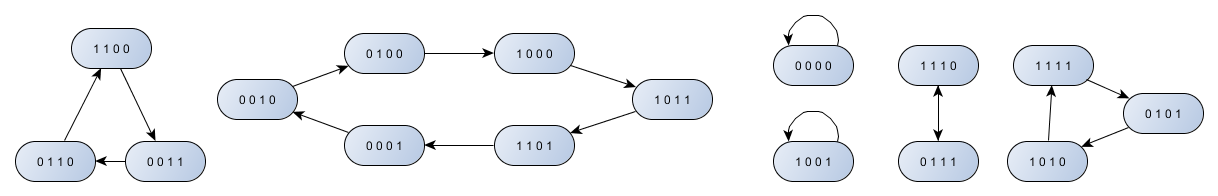
\includegraphics[width=\textwidth]{graf}

\section{}
Známe tedy i schéma v Galoisově tvaru, takže stačí dopočítat vnitřní stavy ($x_0, \dots, x_4$). Víme, že prvních 5 bitů výstupu jsou $11111$. Vždy se tedy k počátečním stavům přičte jednička při posunu nebo ne. Máme tedy rovnice:
$$s_0 = 1 = x_0 \Rightarrow x_0 = 1$$
$$s_1 = 1 = x_1 + 1 \Rightarrow x_1 = 0$$
$$s_2 = 1 = x_2 + 1 \Rightarrow x_2 = 0$$
$$s_3 = 1 = x_3 + 1 + 1 \Rightarrow x_3 = 1$$
$$s_4 = 1 = x_4 + 1 + 1 + 1 \Rightarrow x_4 = 0$$
Počáteční stav v Galoisově módu tedy je $10010$. $x^5+x^4+x^2+x+1$ je sice ireducibilní nad $\mathbb{Z}_2$ ale 1 (primitivní prvek $\mathbb{Z}_2$) není kořenem, takže nemůžeme použít větu. Každopádně po implementaci registru zjistíme, že perioda je stejně ta největší možná a to $2^5-1=31$.

\section{}
Pokud je $x_1 = 0$, tak výsledek odpovídá součinu $x_2 \cdot x_3$. Pokud je $x_1 = 1$, tak výsledek odpovídá skoro (až na poslední řádek, ale to se opraví přičtením již zjistěného $x_2 \cdot x_3$) součtu $x_2+x_3$, takže kandidátem na polynom je $x_1 \cdot (x_2+x_3) + x_2 \cdot x_3 = x_1 \cdot x_2 + x_1 \cdot x_3 + x_2 \cdot x_3$ a ten funguje.
\end{document}